
\begin{figure}[H]
  {
    \setlength{\tabcolsep}{3.0pt}
    \setlength\cmidrulewidth{\heavyrulewidth} % Make cmidrule = 
    \begin{adjustbox}{height=5cm,center}
      \footnotesize
      \begin{tabular}{ll}

        \makecell[l]{
\icode{.BYTE \$00,\$FF,\$00}\\
\icode{.BYTE \$FF,\$00,\$01}
} & \makecell[l]{
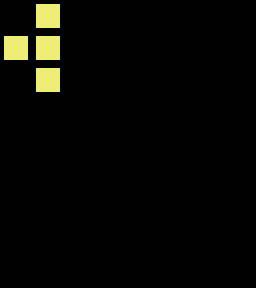
\includegraphics[width=1.3cm]{src/patterns/pixels/pixel_pattern2_0.png}%
} \\
        \midrule

        \makecell[l]{
\icode{.BYTE \$00,\$00}\\
\icode{.BYTE \$02,\$03}
} & \makecell[l]{
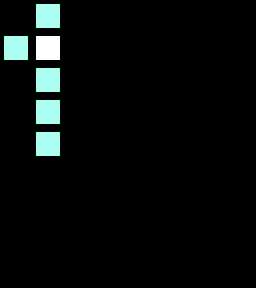
\includegraphics[width=1.3cm]{src/patterns/pixels/pixel_pattern2_1.png}%
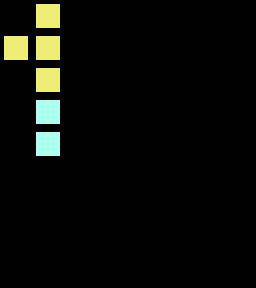
\includegraphics[width=1.3cm]{src/patterns/pixels/pixel_pattern2_2.png}%
} \\
        \midrule

        \makecell[l]{
\icode{.BYTE \$01,\$02,\$03,\$00,\$01,\$02,\$03}\\
\icode{.BYTE \$03,\$03,\$03,\$04,\$04,\$04,\$04}
} & \makecell[l]{
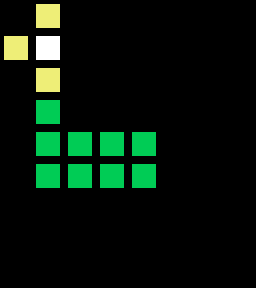
\includegraphics[width=1.3cm]{src/patterns/pixels/pixel_pattern2_3.png}%
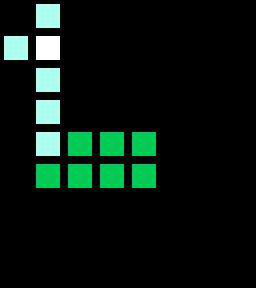
\includegraphics[width=1.3cm]{src/patterns/pixels/pixel_pattern2_4.png}%
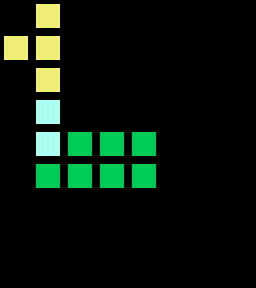
\includegraphics[width=1.3cm]{src/patterns/pixels/pixel_pattern2_5.png}%
} \\
        \midrule

        \makecell[l]{
\icode{.BYTE \$04,\$05,\$06,\$04,\$00,\$01,\$02}\\
\icode{.BYTE \$03,\$02,\$03,\$04,\$05,\$05,\$05}
} & \makecell[l]{
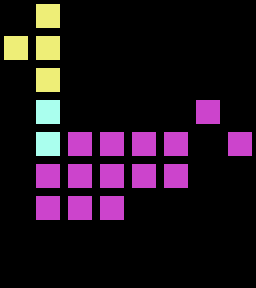
\includegraphics[width=1.3cm]{src/patterns/pixels/pixel_pattern2_6.png}%
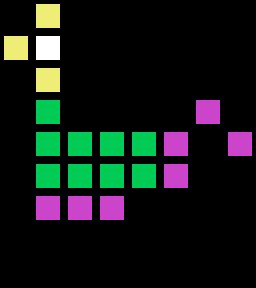
\includegraphics[width=1.3cm]{src/patterns/pixels/pixel_pattern2_7.png}%
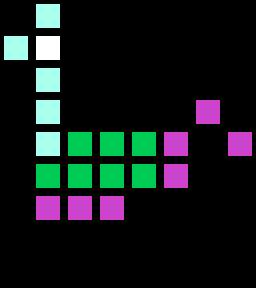
\includegraphics[width=1.3cm]{src/patterns/pixels/pixel_pattern2_8.png}%
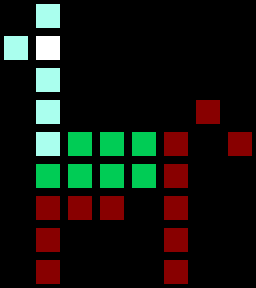
\includegraphics[width=1.3cm]{src/patterns/pixels/pixel_pattern2_9.png}%
} \\
        \midrule

        \makecell[l]{
\icode{.BYTE \$04,\$00,\$04,\$00,\$04}\\
\icode{.BYTE \$05,\$06,\$06,\$07,\$07}
} & \makecell[l]{
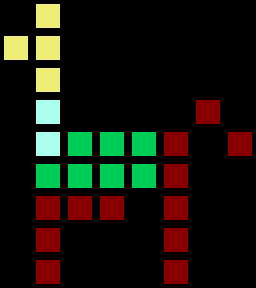
\includegraphics[width=1.3cm]{src/patterns/pixels/pixel_pattern2_10.png}%
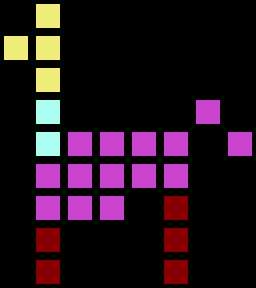
\includegraphics[width=1.3cm]{src/patterns/pixels/pixel_pattern2_11.png}%
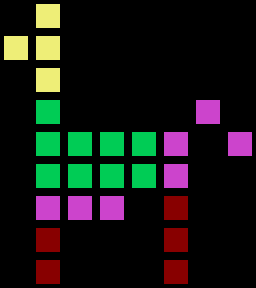
\includegraphics[width=1.3cm]{src/patterns/pixels/pixel_pattern2_12.png}%
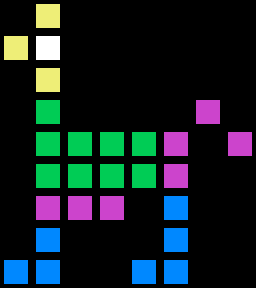
\includegraphics[width=1.3cm]{src/patterns/pixels/pixel_pattern2_13.png}%
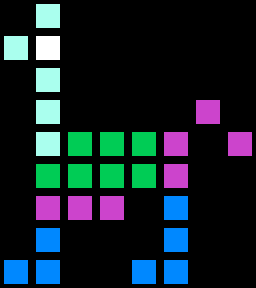
\includegraphics[width=1.3cm]{src/patterns/pixels/pixel_pattern2_14.png}%
} \\
        \midrule

        \makecell[l]{
\icode{.BYTE \$FF,\$03}\\
\icode{.BYTE \$07,\$07}
} & \makecell[l]{
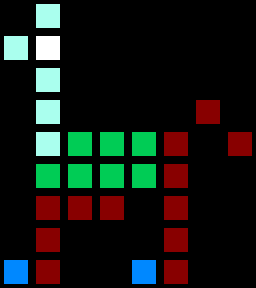
\includegraphics[width=1.3cm]{src/patterns/pixels/pixel_pattern2_15.png}%
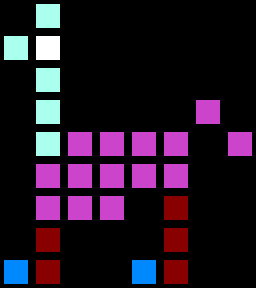
\includegraphics[width=1.3cm]{src/patterns/pixels/pixel_pattern2_16.png}%
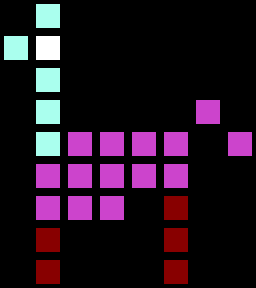
\includegraphics[width=1.3cm]{src/patterns/pixels/pixel_pattern2_17.png}%
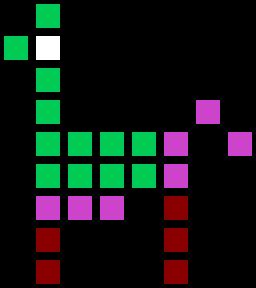
\includegraphics[width=1.3cm]{src/patterns/pixels/pixel_pattern2_18.png}%
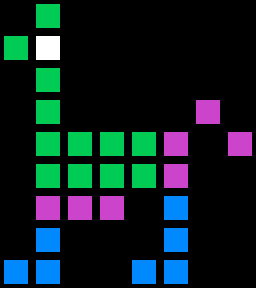
\includegraphics[width=1.3cm]{src/patterns/pixels/pixel_pattern2_19.png}%
} \\
        \midrule

        \makecell[l]{
\icode{.BYTE \$00}\\
\icode{.BYTE \$00}
} & \makecell[l]{
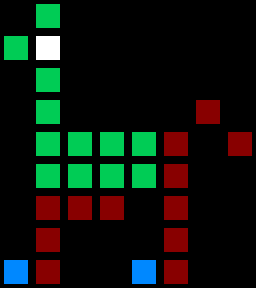
\includegraphics[width=1.3cm]{src/patterns/pixels/pixel_pattern2_20.png}%
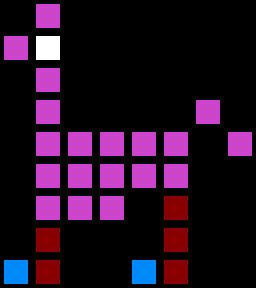
\includegraphics[width=1.3cm]{src/patterns/pixels/pixel_pattern2_21.png}%
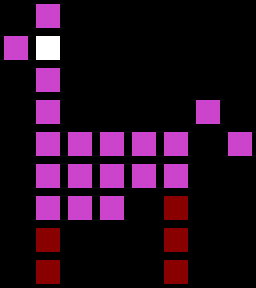
\includegraphics[width=1.3cm]{src/patterns/pixels/pixel_pattern2_22.png}%
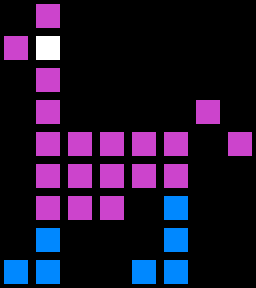
\includegraphics[width=1.3cm]{src/patterns/pixels/pixel_pattern2_23.png}%
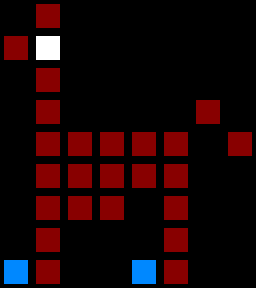
\includegraphics[width=1.3cm]{src/patterns/pixels/pixel_pattern2_24.png}%
} \\
        \midrule

      \end{tabular}
    \end{adjustbox}
  }\caption{The purpose of each of the oscillator values.}
\end{figure}
